\documentclass[11pt]{article}
\usepackage{amsmath}
\usepackage{amssymb}
\usepackage{graphicx}
\usepackage{enumerate}
\usepackage{hyperref}

\pagestyle{plain}
\title{CSCI 4302/5302 Advanced Robotics\\
Assignment 2: Extended Kalman Filter}
\author{Due: 4/11}
\date{}

\begin{document}
\maketitle

\section{Introduction}
In this assignment, you will implement an Extended Kalman Filter (EKF) for robot localization in a continuous world with nonlinear dynamics. The EKF extends the Kalman filter to handle nonlinear systems by linearizing around the current state estimate.

\section{Background}
The EKF maintains a Gaussian belief over continuous states. For a robot in a continuous world:
\begin{itemize}
    \item State space: \((x, y, \theta)\) representing position and orientation
    \item Actions: forward movement and turns with continuous velocities
    \item Measurements: range and bearing to landmarks
\end{itemize}

The filter consists of two main steps:
\begin{enumerate}
    \item Prediction:
    \begin{align*}
        \mu_t &= g(u_t, \mu_{t-1})\\
        \Sigma_t &= G_t\Sigma_{t-1}G_t^T + R_t
    \end{align*}
    where \(G_t\) is the Jacobian of the motion model.
    
    \item Update:
    \begin{align*}
        K_t &= \Sigma_t H_t^T(H_t\Sigma_t H_t^T + Q_t)^{-1}\\
        \mu_t &= \mu_t + K_t(z_t - h(\mu_t))\\
        \Sigma_t &= (I - K_tH_t)\Sigma_t
    \end{align*}
    where \(H_t\) is the Jacobian of the measurement model.
\end{enumerate}

\section{Implementation Tasks}


\subsection{Filter Implementation }
Implement the main filter methods:
\begin{itemize}
    \item Prediction step using linearized motion model
    \item Update step using linearized measurement model
    \item Kalman gain computation
    \item State and covariance updates
\end{itemize}
\emph{Note: } The EKF can be sensitive to tuning. Try to find parameters that allow your filter to track the target well, but do not be concerned if the tracking is poor. This is difficult to localize with just a few lidar beams with nonlinear motion.

\subsection{Analysis and Visualization }
\begin{itemize}
    \item Plot estimated trajectory vs. ground truth
    \item Visualize uncertainty ellipses
    \item Analyze linearization errors
    \item Compare performance with different noise parameters
\end{itemize}

\section{Getting Started}

\subsection{Installation}
Install the package with student dependencies:
\begin{verbatim}
pip install -e .
\end{verbatim}

\subsection{Code Structure}
The template file \texttt{extended\_kalman\_filter.py} contains:
\begin{itemize}
    \item Class definition with required methods
    \item Docstrings explaining expected behavior
    \item TODO comments marking implementation points
    \item Helper functions for matrix operations
\end{itemize}

\subsection{Testing}
Run the provided test suite:
\begin{verbatim}
pytest tests/test_extended_kalman_filter.py -v
pytest tests/test_ekf_vis.py -v
\end{verbatim}

\section{Submission Instructions}
Link to github branch.\\
https://github.com/gyanigk/Advanced-Robotics/tree/homework-5-part-2.gyanigkumar

\begin{figure}[H]
    \centering
    \begin{minipage}[t]{1.0\textwidth}
        \centering
        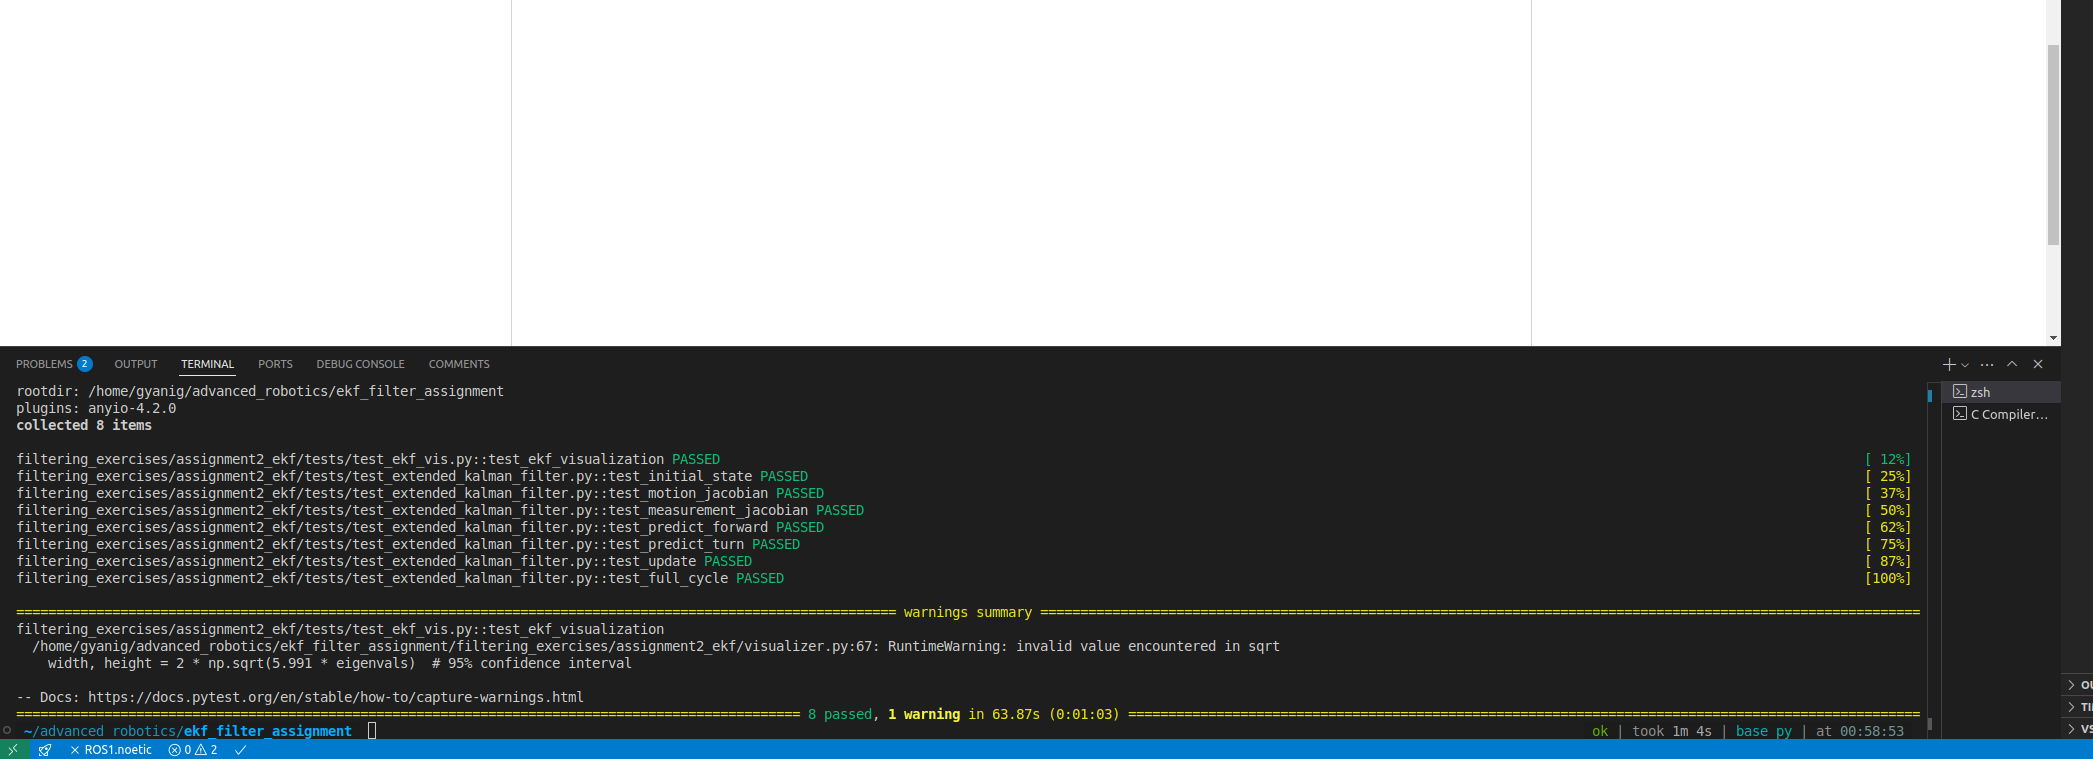
\includegraphics[width=\textwidth]{/home/gyanig/advanced_robotics/ekf_filter_assignment/filtering_exercises/assignment2_ekf/writeup/all_test_passed.png}
        \caption{All tests passed}
        \label{fig:gridworld_v0_det_vi}
    \end{minipage}
\end{figure}


\end{document} 